% !TEX TS-program = pdflatex
% !TEX encoding = UTF-8 Unicode

% This is a simple template for a LaTeX document using the "article" class.
% See "book", "report", "letter" for other types of document.

\documentclass[11pt]{article} % use larger type; default would be 10pt

\usepackage[utf8]{inputenc} % set input encoding (not needed with XeLaTeX)
\usepackage[spanish]{babel}

%%% Examples of Article customizations
% These packages are optional, depending whether you want the features they provide.
% See the LaTeX Companion or other references for full information.

%%% PAGE DIMENSIONS
\usepackage{geometry} % to change the page dimensions
\geometry{a4paper} % or letterpaper (US) or a5paper or....
% \geometry{margin=2in} % for example, change the margins to 2 inches all round
% \geometry{landscape} % set up the page for landscape
%   read geometry.pdf for detailed page layout information

\usepackage{graphicx} % support the \includegraphics command and options
\usepackage[outdir=./]{epstopdf}
% \usepackage[parfill]{parskip} % Activate to begin paragraphs with an empty line rather than an indent
\usepackage{listings}

%%% PACKAGES
\usepackage{booktabs} % for much better looking tables
\usepackage{array} % for better arrays (eg matrices) in maths
\usepackage{paralist} % very flexible & customisable lists (eg. enumerate/itemize, etc.)
\usepackage{verbatim} % adds environment for commenting out blocks of text & for better verbatim
%\usepackage{subfig} % make it possible to include more than one captioned figure/table in a single float
\usepackage{subcaption}
\usepackage{url}
\usepackage{diagbox}
\usepackage{amsmath}
\usepackage{pdfpages}
\usepackage{multirow}
% These packages are all incorporated in the memoir class to one degree or another...

%%% HEADERS & FOOTERS
\usepackage{fancyhdr} % This should be set AFTER setting up the page geometry
\pagestyle{fancy} % options: empty , plain , fancy
\renewcommand{\headrulewidth}{0pt} % customise the layout...
\lhead{}\chead{}\rhead{}
\lfoot{}\cfoot{\thepage}\rfoot{}

%%% SECTION TITLE APPEARANCE
\usepackage{sectsty}
\allsectionsfont{\sffamily\mdseries\upshape} % (See the fntguide.pdf for font help)
% (This matches ConTeXt defaults)

%%% ToC (table of contents) APPEARANCE
\usepackage[nottoc,notlof,notlot]{tocbibind} % Put the bibliography in the ToC
\usepackage[titles,subfigure]{tocloft} % Alter the style of the Table of Contents
\renewcommand{\cftsecfont}{\rmfamily\mdseries\upshape}
\renewcommand{\cftsecpagefont}{\rmfamily\mdseries\upshape} % No bold!

%%% END Article customizations

%%% The "real" document content comes below...

\title{CLP Lab 3 Report}
\author{Albert Aparicio Isarn\\
	\url{albert.aparicio.isarn@alu-etsetb.upc.edu}
	\and 
	Héctor Esteban\\
	\url{hect.esteban@gmail.com}}
\date{} % Activate to display a given date or no date (if empty),
         % otherwise the current date is printed 

\begin{document}
	
	% ---- MATLAB Code definitions ----- %
	\definecolor{mygreen}{rgb}{0,0.6,0}
	\definecolor{mygray}{rgb}{0.5,0.5,0.5}
	\definecolor{mymauve}{rgb}{0.58,0,0.82}
	
	\lstset{ %
		%backgroundcolor=\color{white},   % choose the background color; you must add \usepackage{color} or \usepackage{xcolor}
		basicstyle=\ttfamily\footnotesize,        % the size of the fonts that are used for the code
		breakatwhitespace=false,         % sets if automatic breaks should only happen at whitespace
		breaklines=true,                 % sets automatic line breaking
		captionpos=b,                    % sets the caption-position to bottom
		commentstyle=\color{mygreen},    % comment style
		deletekeywords={...},            % if you want to delete keywords from the given language
		escapeinside={\%*}{*)},          % if you want to add LaTeX within your code
		extendedchars=true,              % lets you use non-ASCII characters; for 8-bits encodings only, does not work with UTF-8
		%frame=single,	                   % adds a frame around the code
		keepspaces=true,                 % keeps spaces in text, useful for keeping indentation of code (possibly needs columns=flexible)
		keywordstyle=\color{blue},       % keyword style
		language=Matlab,                 % the language of the code
		otherkeywords={*,...},            % if you want to add more keywords to the set
		%numbers=left,                    % where to put the line-numbers; possible values are (none, left, right)
		%numbersep=5pt,                   % how far the line-numbers are from the code
		%numberstyle=\tiny\color{mygray}, % the style that is used for the line-numbers
		rulecolor=\color{black},         % if not set, the frame-color may be changed on line-breaks within not-black text (e.g. comments (green here))
		showspaces=false,                % show spaces everywhere adding particular underscores; it overrides 'showstringspaces'
		showstringspaces=false,          % underline spaces within strings only
		showtabs=false,                  % show tabs within strings adding particular underscores
		stepnumber=2,                    % the step between two line-numbers. If it's 1, each line will be numbered
		stringstyle=\color{mymauve},     % string literal style
		tabsize=2,	                   % sets default tabsize to 2 spaces
		title=\lstname                   % show the filename of files included with \lstinputlisting; also try caption instead of title
	}
	
\maketitle

\section{Selección de características con bases de datos gaussianas}

La tabla \ref{tab:select:LC_QC} muestra los errores LC y QC obtenidos en entreno y en test para cada una de las tres dimensiones. La semilla utilizada es la número \textbf{2}.

\begin{table}[h]
	\begin{center}
		\begin{tabular}{| l | c | c | c | c | c | c |}
			\hline
			\textbf{Fase} & \multicolumn{3}{ c |}{\textbf{Training}} & \multicolumn{3}{ c |}{\textbf{Test}} \\
			\hline
			\diagbox[width=11em]{\textbf{Clasificador}}{\textbf{Dimensión}} & \textbf{1D} & \textbf{2D} & \textbf{3D} & \textbf{1D} & \textbf{2D}  & \textbf{3D} \\
			\hline
			\textbf{Lineal (LC)}     & $ 0.00933333 $ & $ 0.01 $       & $ 0.004 $ & $ 0.00533333 $ & $ 0.00533333 $ & $ 0 $ \\
			\hline
			\textbf{Cuadrático (QC)} & $ 0.00466667 $ & $ 0.00133333 $ & $ 0 $     & $ 0.00266667 $ & $ 0 $ & $ 0 $ \\
			\hline
		\end{tabular}
		\caption{Errores LC y QC obtenidos en entreno y en test para cada una de las tres dimensiones. $SNR=10dB$}
		\label{tab:select:LC_QC}
	\end{center}
\end{table}

Con el método MDA y semilla 2, dos proyecciones podrían ser las mostradas en las figuras \ref{fig:select:mda_separate} y \ref{fig:select:mda_overlaid}.

\begin{figure}[h]
	\centering
	\begin{subfigure}[b]{0.435\textwidth}
		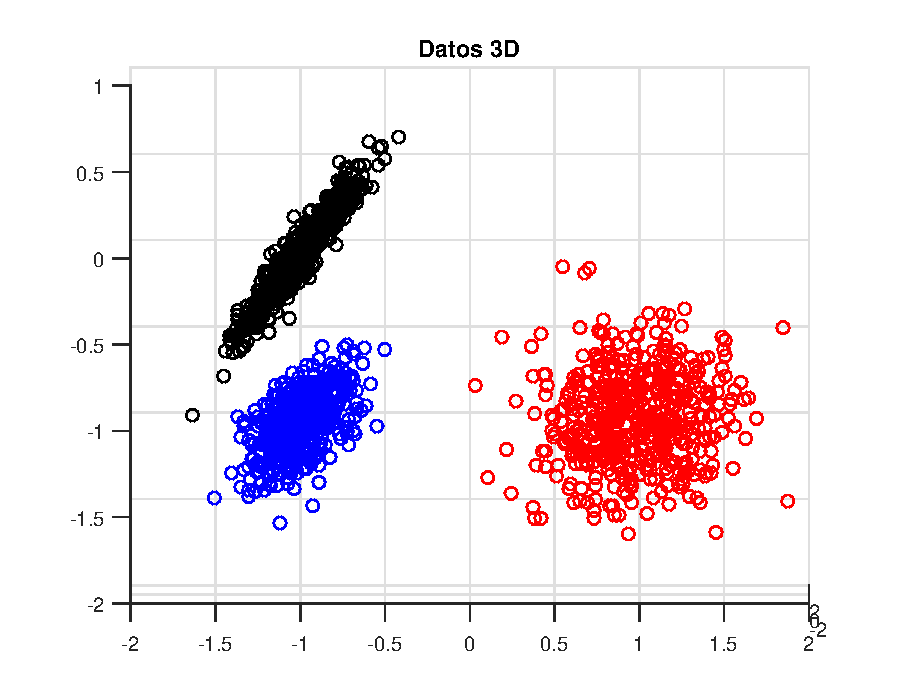
\includegraphics[width=\textwidth]{../21_seleccion/2_mda_separadas.eps}
		\caption[]{\small Proyección 2D con los \emph{clusters} separados.}
		\label{fig:select:mda_separate}
	\end{subfigure}
	\quad
	\begin{subfigure}[b]{0.435\textwidth}
		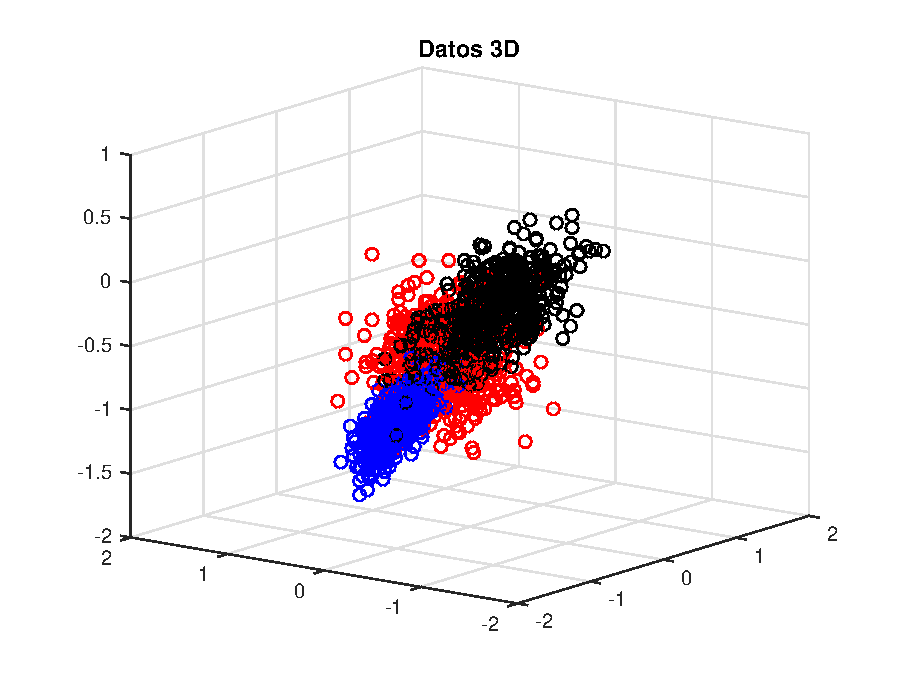
\includegraphics[width=\textwidth]{../21_seleccion/2_mda_juntas.eps}
		\caption[]{\small Proyección 2D con los \emph{clusters} superpuestos.}
		\label{fig:select:mda_overlaid}
	\end{subfigure}
	\caption{Proyecciones 2D para MDA, semilla 2, $SNR=10dB$}
\end{figure}

\clearpage

A continuación se presentan los resultados de los dos apartados anteriores, pero seleccionando $SNR=0dB$.

\begin{table}[h]
	\begin{center}
		\begin{tabular}{| l | c | c | c | c | c | c |}
			\hline
			\textbf{Fase} & \multicolumn{3}{ c |}{\textbf{Training}} & \multicolumn{3}{ c |}{\textbf{Test}} \\
			\hline
			\diagbox[width=11em]{\textbf{Clasificador}}{\textbf{Dimensión}} & \textbf{1D} & \textbf{2D} & \textbf{3D} & \textbf{1D} & \textbf{2D}  & \textbf{3D} \\
			\hline
			\textbf{Lineal (LC)}     & $ 0.194667 $ & $ 0.184 $    & $ 0.156 $     & $ 0.181333 $ & $ 0.154667 $ & $ 0.133333 $ \\
			\hline
			\textbf{Cuadrático (QC)} & $ 0.189333 $ & $ 0.166667 $ & $ 0.0733333 $ & $ 0.157333 $ & $ 0.138667 $ & $ 0.096 $ \\
			\hline
		\end{tabular}
		\caption{Errores LC y QC obtenidos en entreno y en test para cada una de las tres dimensiones. $SNR=0dB$}
		\label{tab:select:0dB:LC_QC}
	\end{center}
\end{table}

Para los casos de 3D, las probabilidades de error son las mismas, ya que el procesado es el mismo (no hay reducción de características). En los casos en que sí se reducen, el MDA da menores probabilidades de error tanto en 2D como en 1D.

\begin{figure}[h]
	\centering
	\begin{subfigure}[b]{0.435\textwidth}
		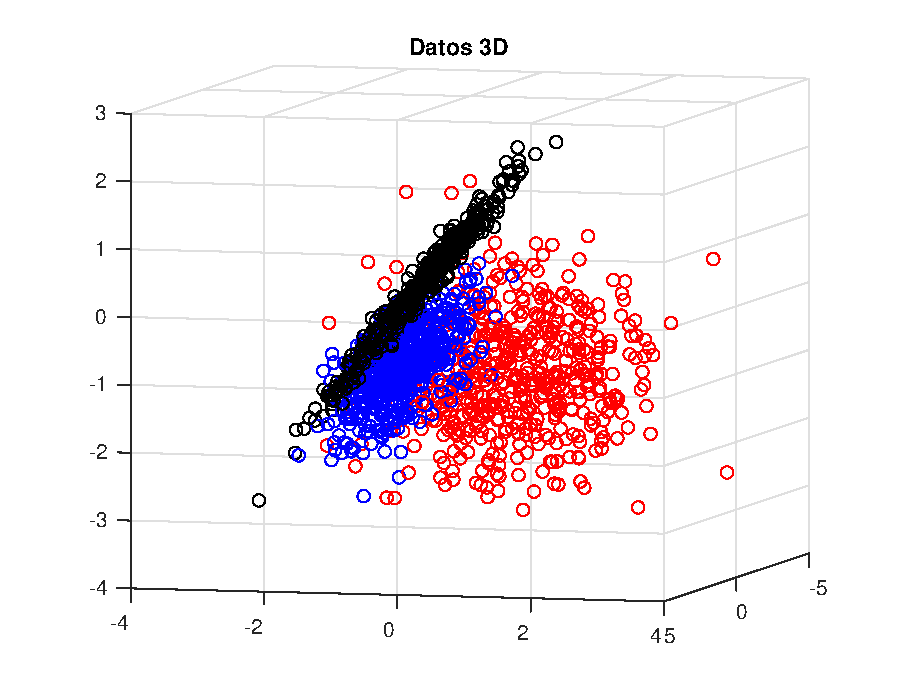
\includegraphics[width=\textwidth]{../21_seleccion/3_mda_0dB_separadas.eps}
		\caption[]{\small Proyección 2D con los \emph{clusters} separados.}
		\label{fig:select:0dB:mda_separate}
	\end{subfigure}
	\quad
	\begin{subfigure}[b]{0.435\textwidth}
		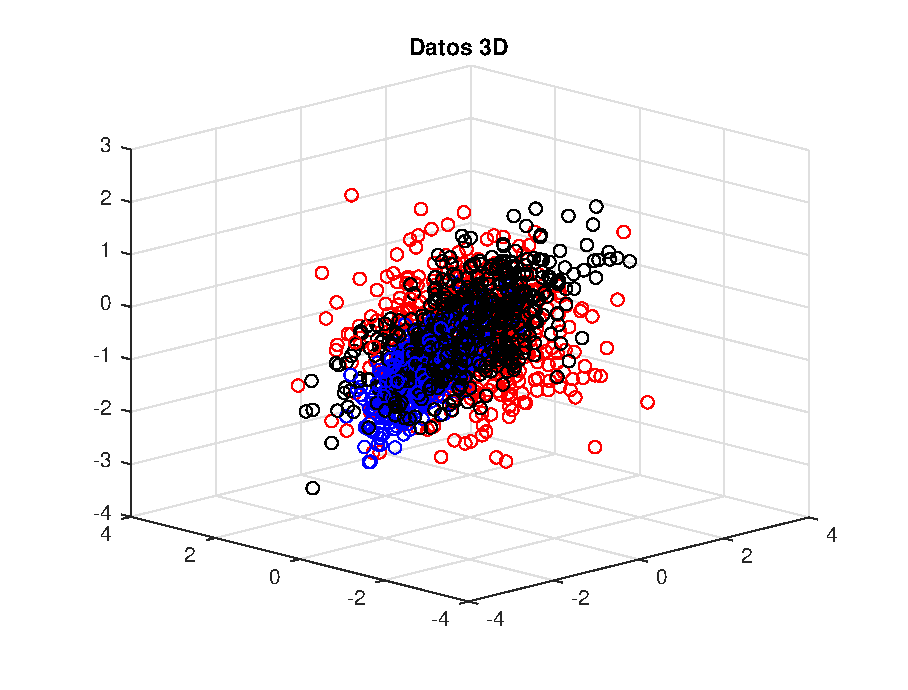
\includegraphics[width=\textwidth]{../21_seleccion/3_mda_0dB_superpuestas.eps}
		\caption[]{\small Proyección 2D con los \emph{clusters} superpuestos.}
		\label{fig:select:0dB:mda_overlaid}
	\end{subfigure}
	\caption{Proyecciones 2D para MDA, semilla 2, $SNR=0dB$}
\end{figure}

En las figuras \ref{fig:select:0dB:pca:scatter} y \ref{fig:select:0dB:mda:scatter} se muestran los \emph{scatters} para los métodos PCA y MDA para 1 y 2 dimensiones.

Para 1D, el MDA compacta mejor los datos, reduciendo la superposición de los datos. El PCA muestra los datos muy superpuestos.

En el caso 2D, todas las clases están superpuestas, aunque en MDA lo están en menor grado. Además, en MDA las clases están más compactadas. En el scatter de PCA, hay mayor dispersión de datos.

\begin{figure}[h]
	\centering
	\begin{subfigure}[b]{0.435\textwidth}
		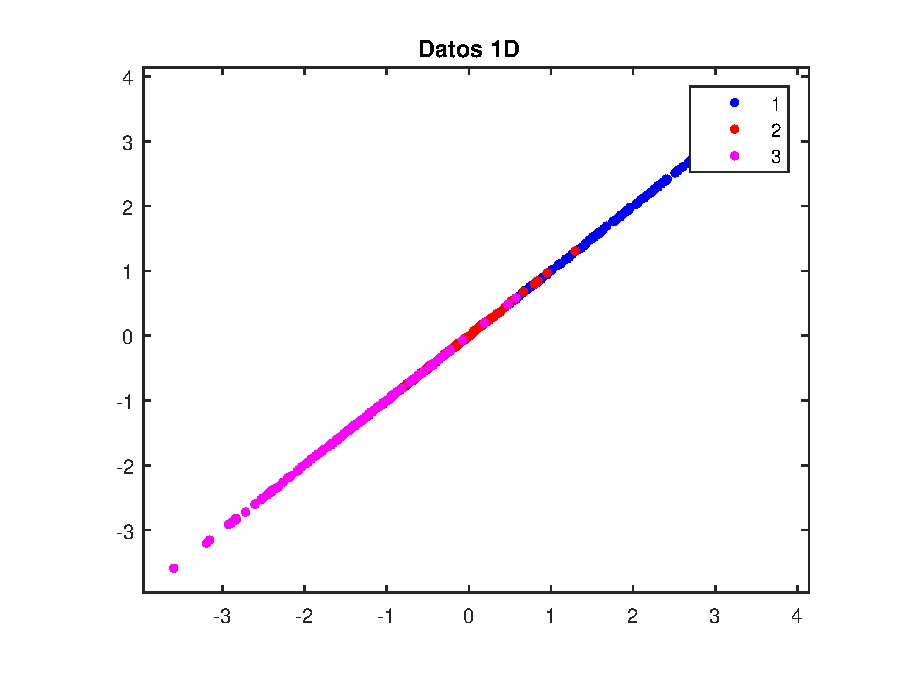
\includegraphics[width=\textwidth]{../21_seleccion/3_pca_0dB_1d.eps}
		\caption[]{\small Proyección en 1D.}
		\label{fig:select:0dB:pca:scatter:1D}
	\end{subfigure}
	\quad
	\begin{subfigure}[b]{0.435\textwidth}
		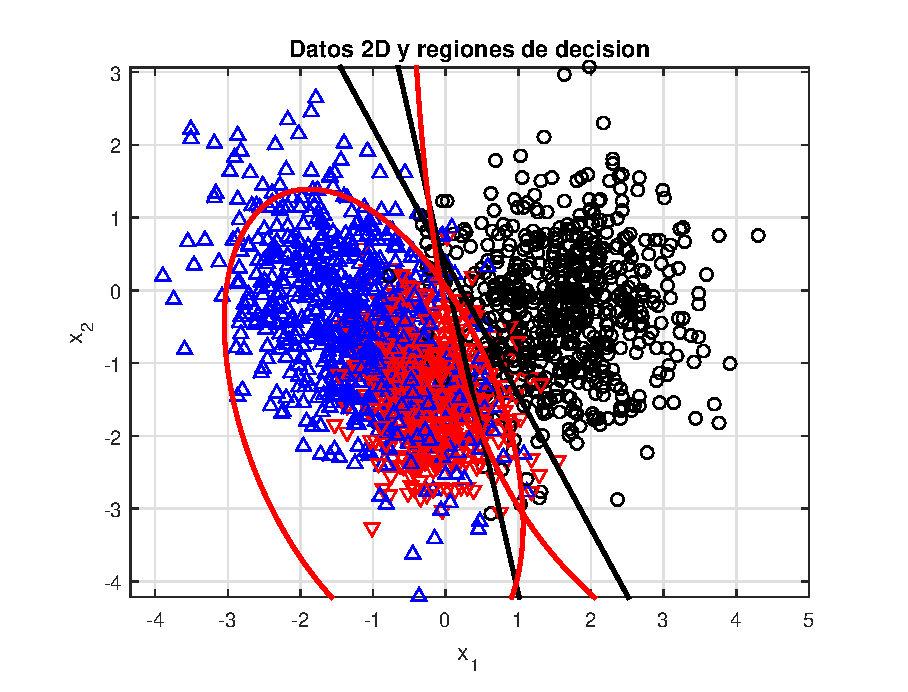
\includegraphics[width=\textwidth]{../21_seleccion/3_pca_0dB_2d.eps}
		\caption[]{\small Proyección en 2D.}
		\label{fig:select:0dB:pca:scatter:2D}
	\end{subfigure}
	\caption{Proyecciones en 1D y 2D para PCA, semilla 2, $SNR=0dB$}
	\label{fig:select:0dB:pca:scatter}
\end{figure}

\begin{figure}[h]
	\centering
	\begin{subfigure}[b]{0.435\textwidth}
		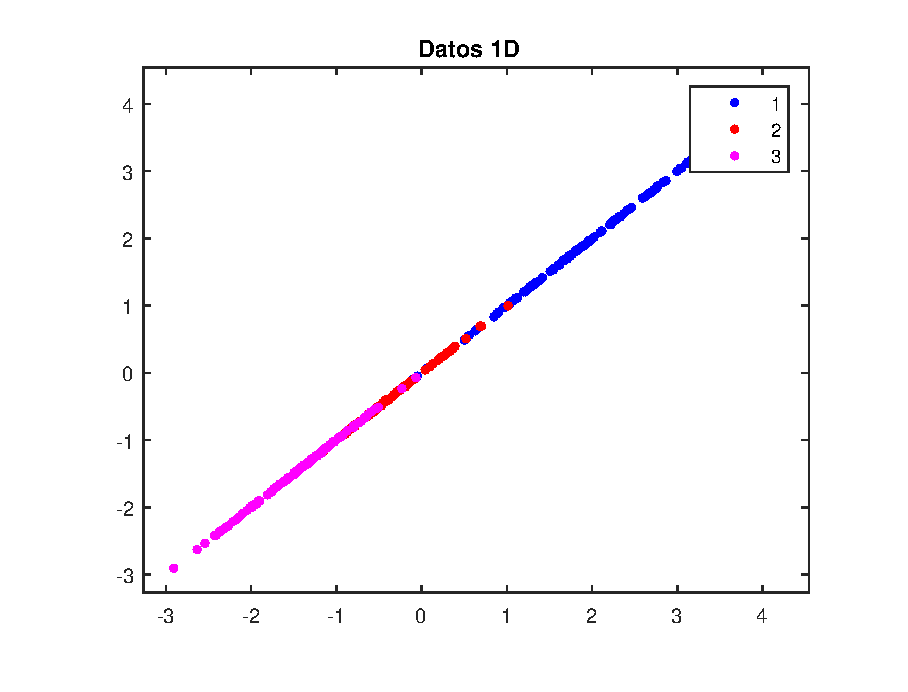
\includegraphics[width=\textwidth]{../21_seleccion/3_mda_0dB_1d.eps}
		\caption[]{\small Proyección en 1D.}
		\label{fig:select:0dB:mda:scatter:1D}
	\end{subfigure}
	\quad
	\begin{subfigure}[b]{0.435\textwidth}
		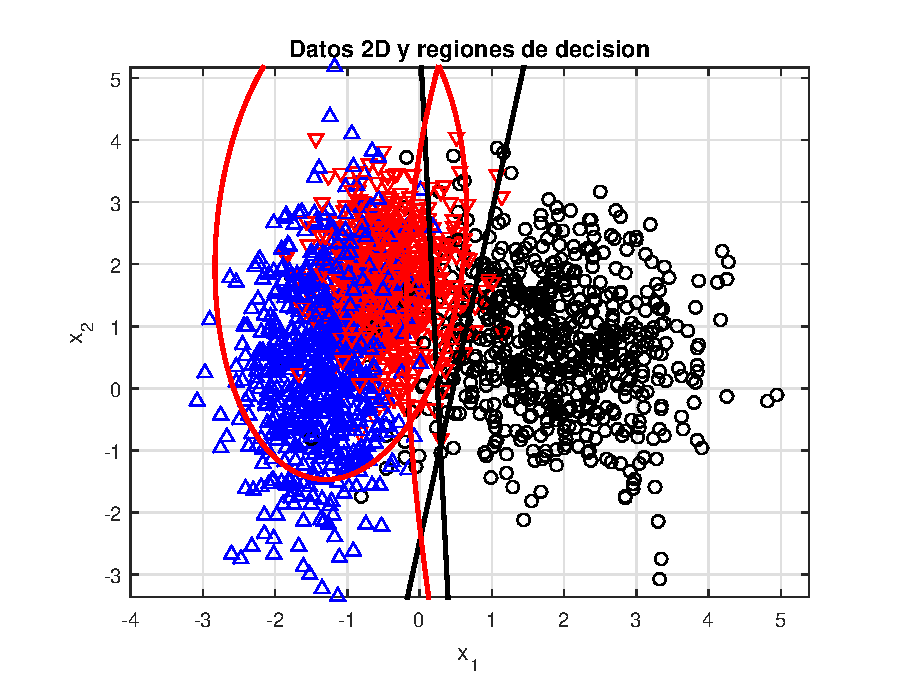
\includegraphics[width=\textwidth]{../21_seleccion/3_mda_0dB_2d.eps}
		\caption[]{\small Proyección en 2D.}
		\label{fig:select:0dB:mda:scatter:2D}
	\end{subfigure}
	\caption{Proyecciones en 1D y 2D para MDA, semilla 2, $SNR=0dB$}
	\label{fig:select:0dB:mda:scatter}
\end{figure}

A continuación se presentan los resultados del apartado 4 y 5 de la práctica, usando distribuciones gausianas con las medias alineadas.

Usando la semilla 2, los vectores de las medias son los que se muestran en la ecuación \eqref{eq:4:means}:

\begin{equation} \label{eq:4:means}
\left( \begin{array}{ccc}
0.99631702257037136 & -0.013479105534217606 & -0.084680010926471622 \\
0 & 0 & 0 \\
-0.99631702257037136 & 0.013479105534217606 & 0.084680010926471622 \\
\end{array} \right)
\end{equation}

El rango de la matriz $S_b$ teóricamente deberia ser 1 porque las medias están alineadas. Sin embargo, MATLAB da como resultado 2, debido a la estimación de las medias. Usando MDA, con 1 característica bastaria.

\clearpage

A continuación se presentan los resultados de los apartados iniciales, usando $SNR = \left\lbrace-5, 5 \right\rbrace dB$.

Las probabilidades de error de los clasificadores LC y QC se muestran en las tablas \ref{tab:5dB:LC_QC} y \ref{tab:-5dB:LC_QC}

\begin{table}[h]
	\begin{center}
		\begin{tabular}{| l | c | c | c | c | c | c |}
			\hline
			\textbf{Fase} & \multicolumn{3}{ c |}{\textbf{Training}} & \multicolumn{3}{ c |}{\textbf{Test}} \\
			\hline
			\diagbox[width=11em]{\textbf{Clasificador}}{\textbf{Dimensión}} & \textbf{1D} & \textbf{2D} & \textbf{3D} & \textbf{1D} & \textbf{2D}  & \textbf{3D} \\
			\hline
			\textbf{Lineal (LC)}     & $ 0 $ & $ 0 $       & $ 0 $ & $ 0 $ & $ 0 $ & $ 0 $ \\
			\hline
			\textbf{Cuadrático (QC)} & $ 0 $ & $ 0 $ & $ 0 $     & $ 0 $ & $ 0 $ & $ 0 $ \\
			\hline
		\end{tabular}
		\caption{Errores LC y QC obtenidos en entreno y en test para cada una de las tres dimensiones. $SNR=5dB$. Se ha usado la semilla 3}
		\label{tab:5dB:LC_QC}
	\end{center}
\end{table}

\begin{table}[h]
	\begin{center}
		\begin{tabular}{| l | c | c | c | c | c | c |}
			\hline
			\textbf{Fase} & \multicolumn{3}{ c |}{\textbf{Training}} & \multicolumn{3}{ c |}{\textbf{Test}} \\
			\hline
			\diagbox[width=11em]{\textbf{Clasificador}}{\textbf{Dimensión}} & \textbf{1D} & \textbf{2D} & \textbf{3D} & \textbf{1D} & \textbf{2D}  & \textbf{3D} \\
			\hline
			\textbf{Lineal (LC)}     & $ 0.674 $ & $ 0.660667 $ & $ 0 $ & $ 0.674667 $ & $ 0.666667 $ & $ 0 $ \\
			\hline
			\textbf{Cuadrático (QC)} & $ 0.67 $  & $ 0.658667 $ & $ 0 $ & $ 0.650667 $ & $ 0.658667 $ & $ 0 $ \\
			\hline
		\end{tabular}
		\caption{Errores LC y QC obtenidos en entreno y en test para cada una de las tres dimensiones. $SNR=-5dB$. Se ha usado la semilla 3}
		\label{tab:-5dB:LC_QC}
	\end{center}
\end{table}

En las figuras \ref{fig:5dB:mda_proj} y \ref{fig:-5dB:mda_proj} se muestran las proyecciones 2D para el método MDA.

El método MDA resulta ventajoso cuando hay poca separación entre clases, de manera que a la hora de reducir características, se trata de maximizar esta separación.

\begin{figure}[h]
	\centering
	\begin{subfigure}[b]{0.435\textwidth}
		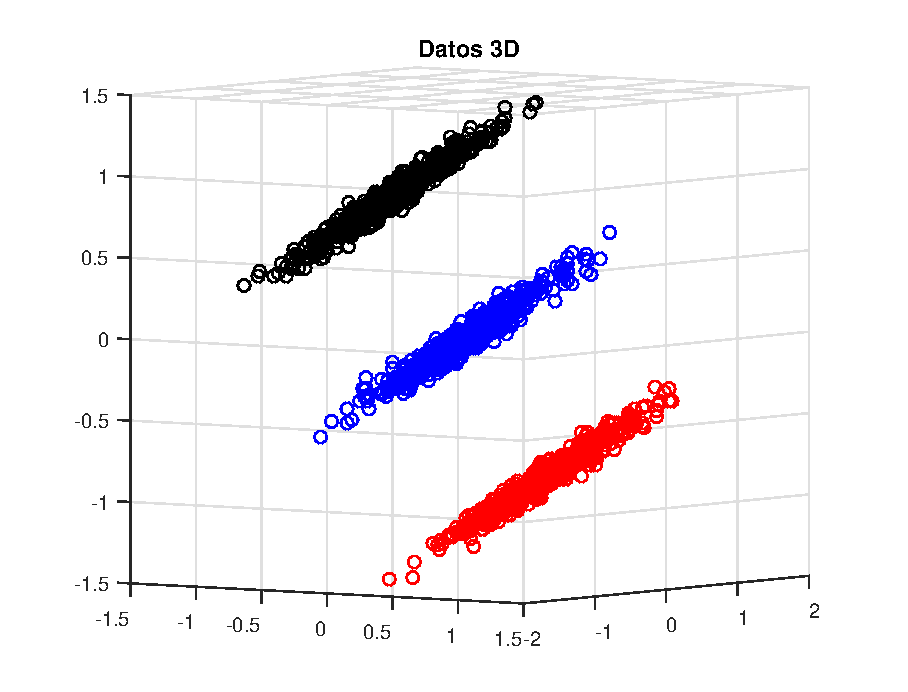
\includegraphics[width=\textwidth]{../21_seleccion/51_mda_5dB_separadas.eps}
		\caption[]{\small Proyección 2D con los \emph{clusters} separados.}
		\label{fig:5dB:mda_proj:separated}
	\end{subfigure}
	\quad
	\begin{subfigure}[b]{0.435\textwidth}
		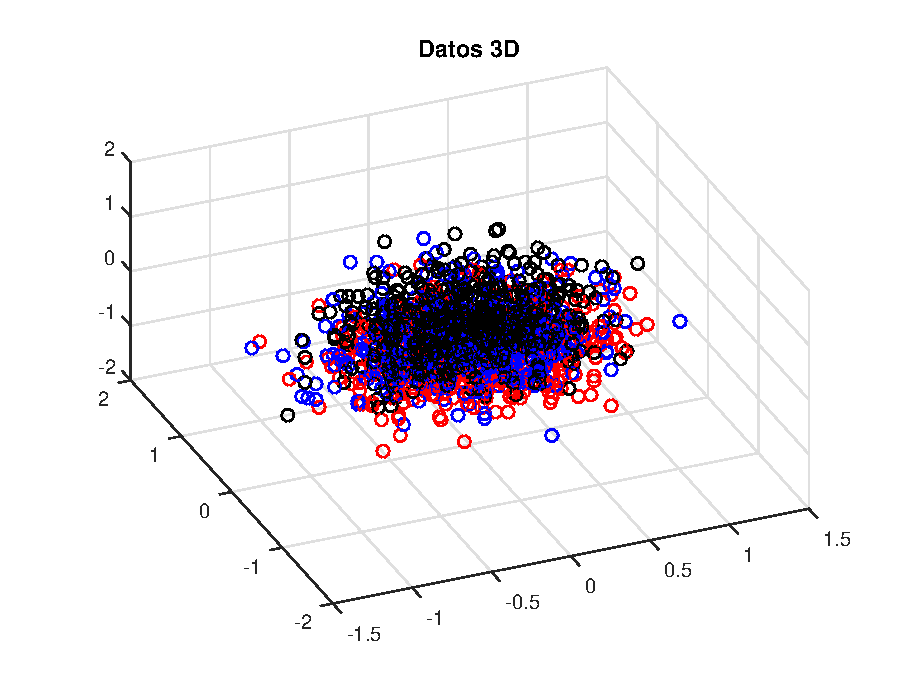
\includegraphics[width=\textwidth]{../21_seleccion/51_mda_5dB_superpuestas.eps}
		\caption[]{\small Proyección 2D con los \emph{clusters} superpuestos.}
		\label{fig:5dB:mda_proj:overlapped}
	\end{subfigure}
	\caption{Proyecciones 2D para MDA, semilla 3, $SNR=5dB$}
	\label{fig:5dB:mda_proj}
\end{figure}

\begin{figure}[h]
	\centering
	\begin{subfigure}[b]{0.435\textwidth}
		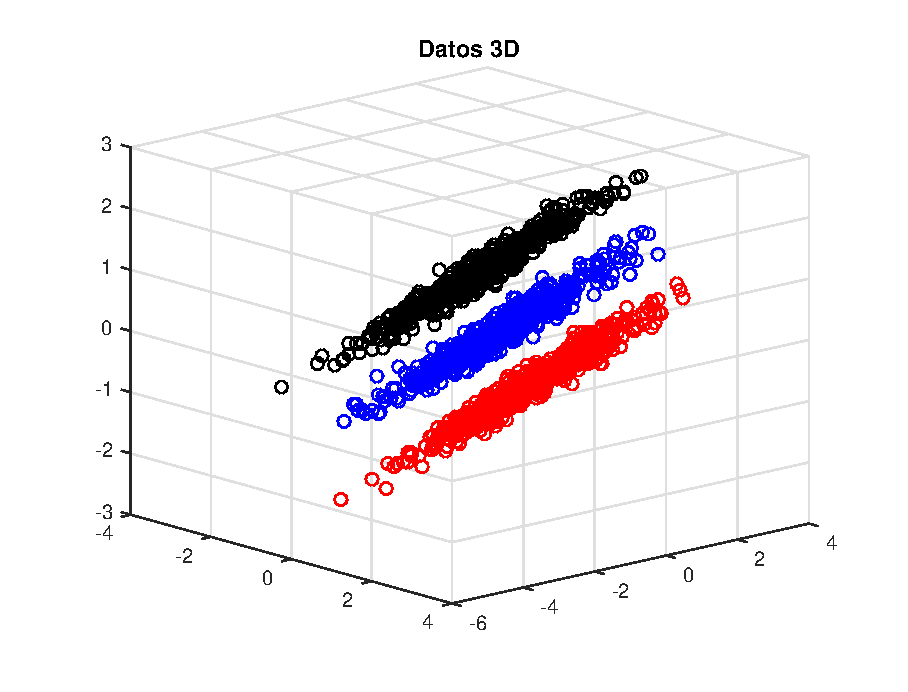
\includegraphics[width=\textwidth]{../21_seleccion/5_mda_m5dB_separadas.eps}
		\caption[]{\small Proyección 2D con los \emph{clusters} separados.}
		\label{fig:-5dB:mda_proj:separated}
	\end{subfigure}
	\quad
	\begin{subfigure}[b]{0.435\textwidth}
		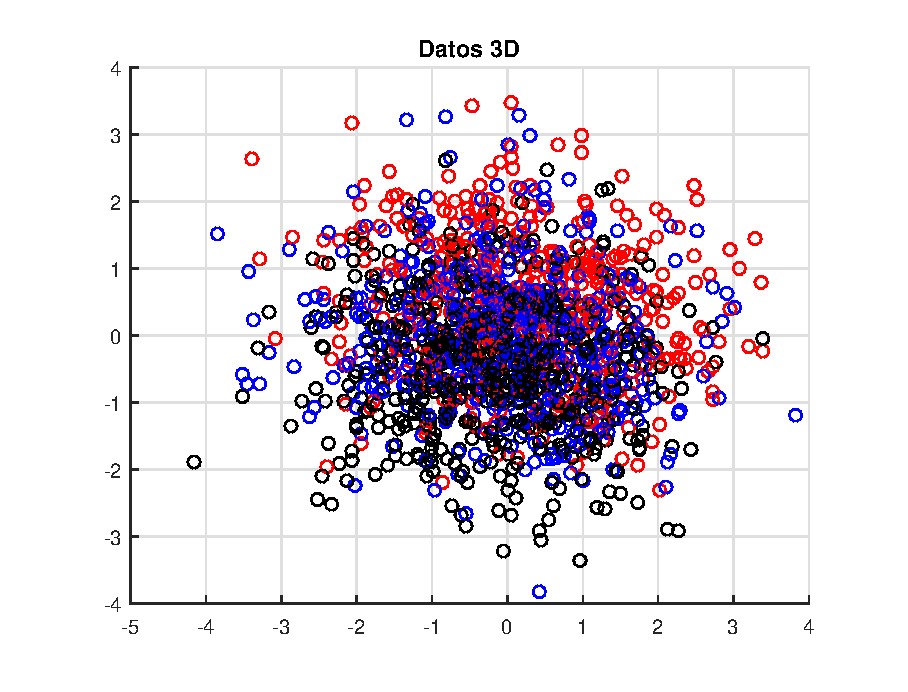
\includegraphics[width=\textwidth]{../21_seleccion/51_mda_m5dB_superpuestas.eps}
		\caption[]{\small Proyección 2D con los \emph{clusters} superpuestos.}
		\label{fig:-5dB:mda_proj:overlapped}
	\end{subfigure}
	\caption{Proyecciones 2D para MDA, semilla 3, $SNR=-5dB$}
	\label{fig:-5dB:mda_proj}
\end{figure}

\clearpage

\section{MDA en clasificación}

El gráfico de los errores de clasificación para $d'=1:256$ se muestra en la figura \ref{fig:mda:256}.


\begin{figure}[h]
	\centering
	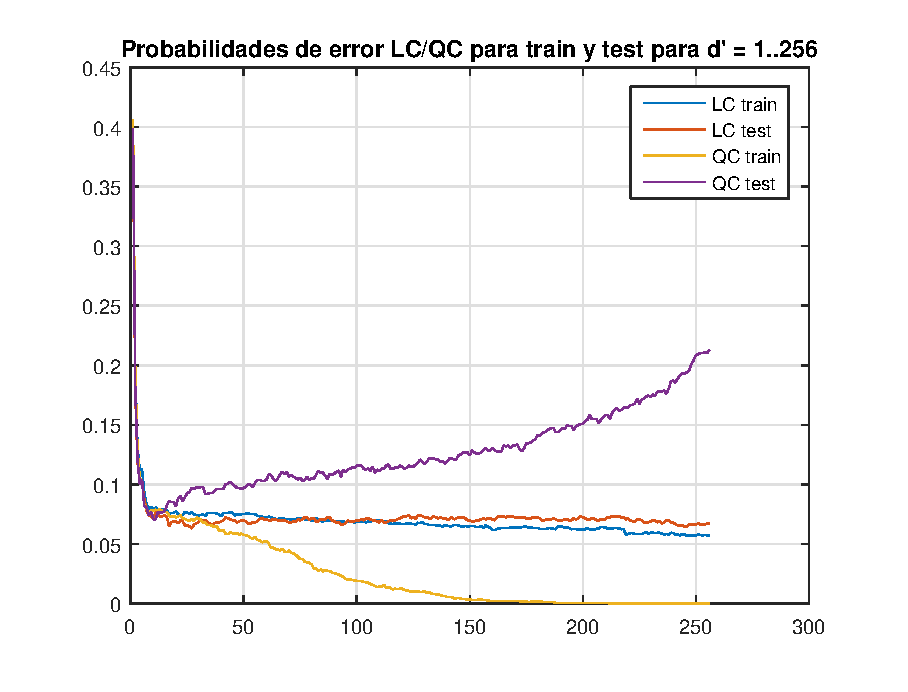
\includegraphics[width=\textwidth]{../22_mda/prob_error_pca.eps}
	\caption[]{\small Gráficos de los errores de clasificación para $d'=1:256$.}
	\label{fig:mda:256}
\end{figure}

Para usar el método MDA, $d_{MAX}$ será 4, ya que MDA puede trabajar hasta c-1 (c numero de clases). Hemos visto que esto se da en el momento de calcular la matriz W, ya que tiene tamaño 256x4

Los gráficos de los errores de clasificación, para $d'=1:d_{MAX}$, para los métodos PCA y MDA se muestran en las figuras \ref{fig:mda:dmax:pca} y \ref{fig:mda:dmax:mda}.

Las probabilidades de error son menores en MDA, para $d'=1:4$.

\clearpage

\begin{figure}[h]
	\centering
	\begin{subfigure}[b]{\textwidth}
		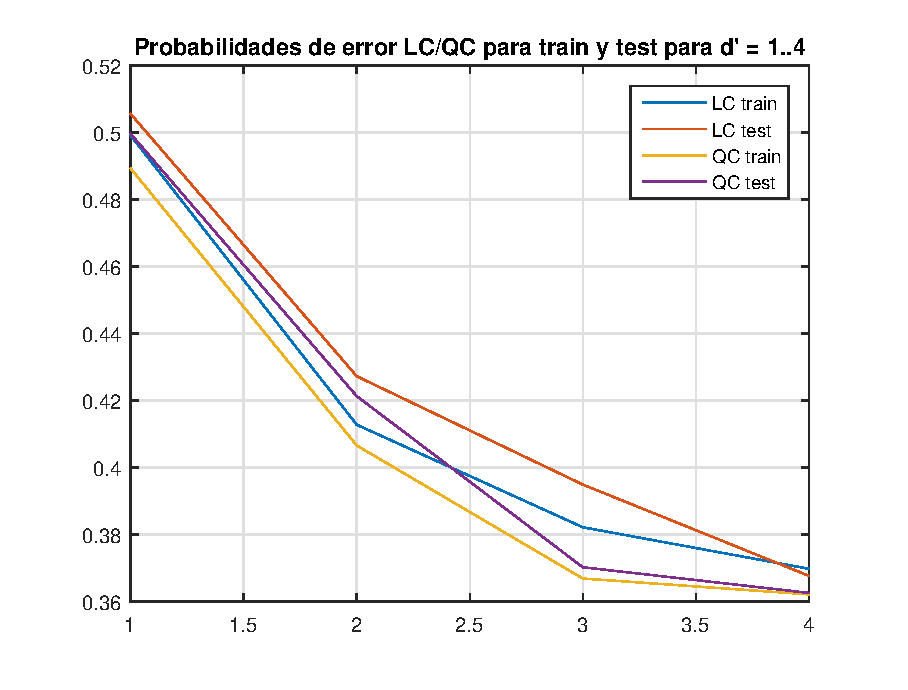
\includegraphics[width=\textwidth]{../22_mda/prob_error_pca_1_4.eps}
		\caption[]{\small Método PCA}
		\label{fig:mda:dmax:pca}
	\end{subfigure}

	\begin{subfigure}[b]{\textwidth}
		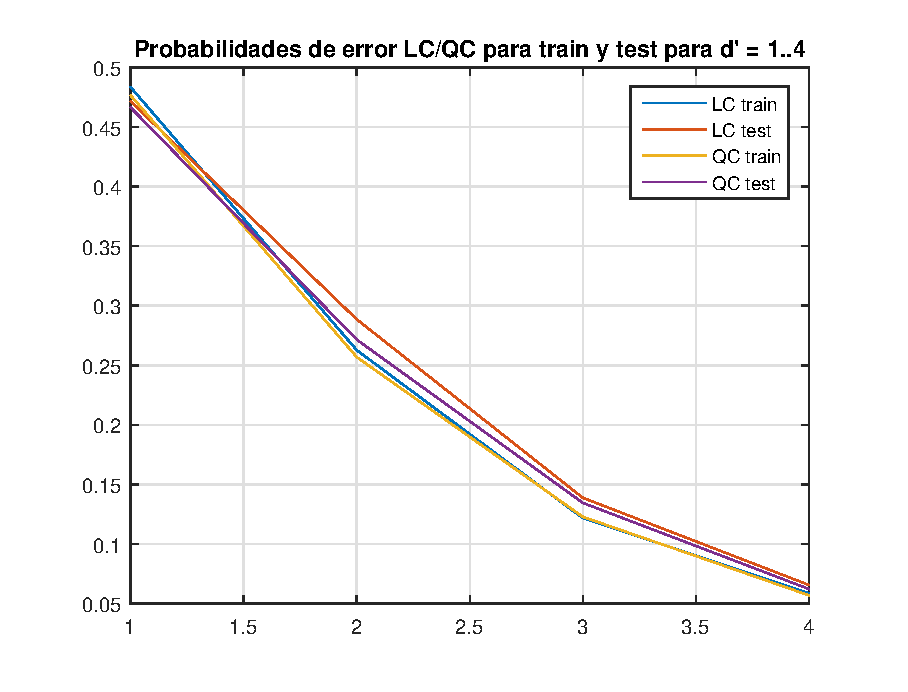
\includegraphics[width=\textwidth]{../22_mda/prob_error_mda.eps}
		\caption[]{\small Método MDA}
		\label{fig:mda:dmax:mda}
	\end{subfigure}
	\caption{Gráficos de errores de clasificación para $d'=1:4$ con los métodos PCA y MDA.}
	\label{fig:mda:dmax}
\end{figure}

\clearpage

Código fuente de \texttt{prac3\_fonemas\_MDA.m}

\lstinputlisting{../prac3_fonemas_MDA.m}

\end{document}
